\section{Data / MC Samples}\label{sec:DataSamples}

This section outlines the data and Monte Carlo sets used in this analysis. \\
For the data, we are using a set which spans all of Run-II positive polarity data. Details on this sample can be found in Section \ref{sec:data}. For the simulation, we use the G4Beamline Monte Carlo (Section \ref{sec:G4Beamline}) and the Data Driven single particle Monte Carlo (DDMC, Section \ref{sec:DDMCSamples}). 


%%%%%%%%%%%%%%%%%%%%%%%%%%%%%%%%%%%%%%%%%%%%%%
\subsection{Data}\label{sec:data}
%%%%%%%%%%%%%%%%%%%%%%%%%%%%%%%%%%%%%%%%%%%%%%



LArIAT successfully ran for 9 weeks in 2015 (Run I) and 24 weeks in 2016 (Run II). Some spectacular Kaon interactions were found in data from Run I (see Figure \ref{fig:MCdata} and its great agreement with the MC),
but the Kaon statistics in Run I is not enough to perform a cross section analysis. Figure \ref{fig:BeamComp} shows the reason behind the low statistics: this figure represents the tertiary beam composition of one of the first data runs. Two aspects of this plot are particularly notable. Firstly, Kaons are very few in the beam. However, the few Kaons produced are in the correct range of momentum for proton decay studies (compare the momentum on Figure \ref{fig:KGenie}).  LArIAT Run II provides enough statistic to measure Kaon cross section. 
\begin{figure}[hpbt]
\centering
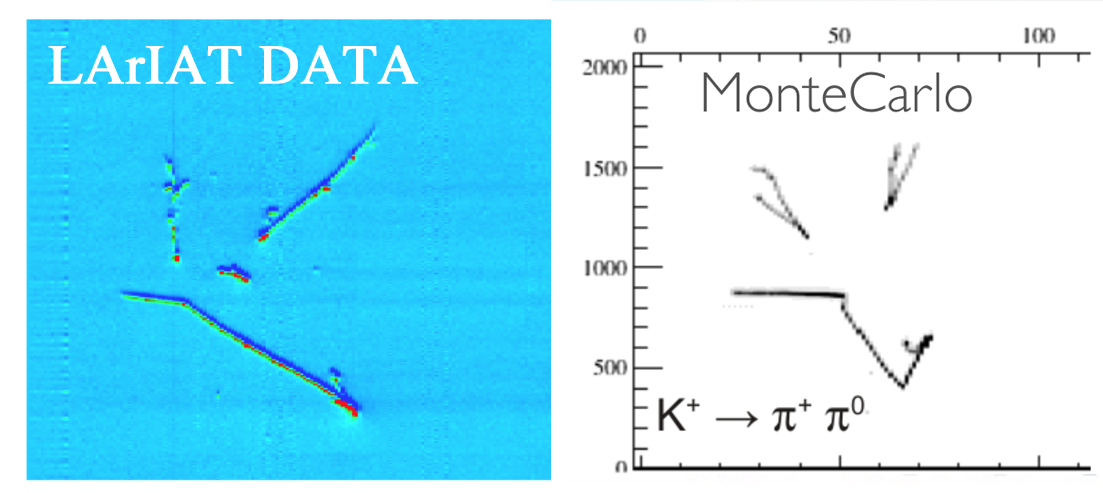
\includegraphics[width=6in]{images/Lariat/KDataMC}
\caption{Direct comparson between a Kaon event in LArIAT Run I data and in LArIAT MC. }
\label{fig:MCdata}
\end{figure}


\begin{figure}[h!]
\centering
\begin{minipage}{0.45\textwidth}
\centering
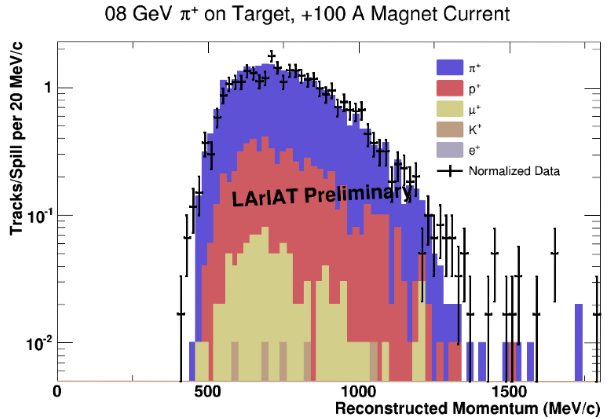
\includegraphics[width=3.5in]{images/Lariat/Beam}
\caption{Particle spectrum at the TPC produced with the LArIAT 8 GeV tertiary beam.}
\label{fig:BeamComp}
\end{minipage}\hfill
\centering
\begin{minipage}{0.45\textwidth}
\centering
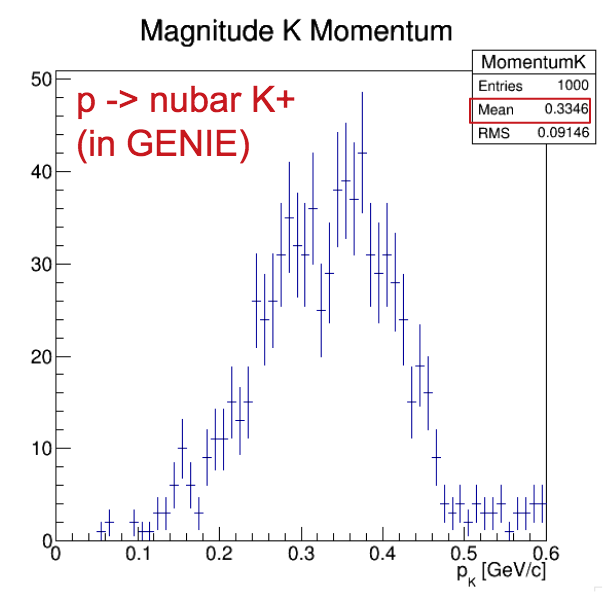
\includegraphics[width=3in]{images/Lariat/KaonGenie}
\caption{Momentum distribution for the Kaon in the $p \rightarrow K^{+} \bar\nu$ mode proton decay as simulated by GENIE.}
\label{fig:KGenie}
\end{minipage}
\end{figure}




The Run-II data use the definitions \href{https://redmine.fnal.gov/redmine/projects/lardbt/wiki/Recommended_SAM_Datasets}{oulined on this Wiki page} and summarized in Table \ref{tab:datasamples}.

\begin{center}
\begin{table}[htb]
	\begin{center}
	%\resizebox{0.95\textwidth}{!}{%
	\begin{tabular}{|c|c|c|}
	\multicolumn{3}{c}{\textbf{Summary of Data Samples}} \\
	\hline \hline
	 Run Period & Data Set Definition & Samweb Meaning \\
%	\hline
%	 &  & \verb!defname: TPC_voltages_nominal! \\
%	\hline
%	 &  & \verb!TPC_MaxGainAndFilter! \\
%	\hline
%	Run-I & \verb!Lovely1_Neg_RunI_elenag_v02! & \verb!TPC_nominal_read_out_and_timing!  \\
%	\hline
%	 & & \verb!BothTOF_OnAndReadOut!  \\
%	\hline
%	 & & \verb!AllMWPC_OnAndReadOut!  \\
%	 \hline
%	 & & \verb!lariat_mid_f_mc7anb < 0! \\
%	\hline
%	\line
%	 & & \verb!run_number >= 8000 and run_number <= 10226! \\
     \hline	
	&  & \verb!defname: TPC_voltages_nominal! \\
	\hline
	 &  & \verb!TPC_MaxGainAndFilter! \\
	\hline
	Run-II & \verb!Lovely1_Pos_RunII_elenag_v04! & \verb!TPC_nominal_read_out_and_timing!  \\
	\hline
	 & & \verb!BothTOF_OnAndReadOut!  \\
	\hline
	 & & \verb!AllMWPC_OnAndReadOut!  \\
	 \hline
	 & & \verb!lariat_mid_f_mc7anb > 0! \\
	 	 \hline
	 & & \verb!create_date < '2017-06-02'! \\

	 \hline
	\end{tabular}%}
	\caption{Summary of the data samples used for this analysis. }
	\label{tab:datasamples}
	\end{center}
\end{table}
\end{center}

The relevant Samweb definitions listed in Table \ref{tab:datasamples} which require some explaining are defined as:

\begin{itemize}
\item \textbf{TPC Voltages Nominal}: Requires the cathode to be at greater than 23 kV, the collection plane wires voltage to be between 320 and 350 V, the induction plane voltage to be between -10 and -20 V, and the shield plane voltage to be greater than -310 V

\item \textbf{TPC MaxGainAndFilter}: Requires the ASIC configuration to be set as ``3'' for both the filter and the gain setting

\item \textbf{TPC Nominal Read Out and Timing}: Requires the readout of the TPC was enabled, the recorded number of time ticks is 3072, and the delay of 36900 was set on the v1495 (trigger card).
\item \textbf{lariat\_mid\_f\_mc7anb \textgreater 0} : Requires the polarity of the magnets to be positive
\item \textbf{create\_date \textless  2017-06-02}: Avoids the introduction of run 3 data and newly sliced data
\end{itemize}


It is important to provide a break down of the beam conditions for the period of data taking because the beam composition, hence the kaon content, varies according to the energy of the secondary beam and the strength of the magnetic field inside the magnets. Table \ref{tab:beamConditions} shows a break down of the beam conditions for both the beam data selected by  \verb!Lovely1_Pos_RunII_elenag_v04! and the events that pass the kaon candidates selection.


\begin{table}[]
\centering
\caption{Break down of beam conditions for Run-II positive polarity. $I$ is the value of the current in the magnets and $E$ is the energy of the secondary beam.  }
\label{tab:beamConditions}
\begin{tabular}{l|l|l|l|l|}
\cline{2-5}
                                       & \multicolumn{2}{l|}{Lovely1\_Pos\_RunII\_elenag\_v04} & \multicolumn{2}{l|}{Kaon candidate sample} \\ \cline{2-5} 
                                       & Run \% & Event \% & Run \% & Event \% \\ \hline
\multicolumn{1}{|l|}{I = + 100 A, E = 64 GeV}   &   61.8          &        75.0   & 75.1  &  90.35   \\ \hline
\multicolumn{1}{|l|}{I =   + 60 A, E = 64 GeV}   &    30.1         &         23.8  & 24.9  &   9.65     \\ \hline
\multicolumn{1}{|l|}{Info not available}              &      8.1         &           1.2   &    0.0 &       0.0               \\ \hline
\end{tabular}
\end{table}



%%%%%%%%%%%%%%%%%%%%%%%%%%%%%%%%%%%%%%%%%%%%%%%%%%%%%%%%%%%%
\subsection{Monte Carlo Samples}\label{sec:MCSamples}
For the simulation of the tertiary beam, we use a combination of two MC generators: the G4Beamline Monte Carlo and the Data Driven single particle Monte Carlo (DDMC).   We use the G4Beamline MC to calculate the particle composition of the beam just before the cryostat. In order to simulate the beam line particles after Wire-Chamber 4, we use the DDMC. 

\subsubsection{G4Beamline }\label{sec:G4Beamline}
At the moment of this writing,  G4Beamline simulates transportation of particles through the beam line from the LArIAT target until ``Big Disk'', a fictional, void detector located just before the cryostat. The responses of  the beam line detector are not simulated. 

The two beam conditions relevant for this analysis are simulated: secondary beam energy of 64 GeV, positive polarity magnet with current of 100 A and 60 A. Figure \ref{fig:beamspectrum} shows the tertiary beam spectra for the 64 GeV and 100 A condition on the left and for the 64 GeV and 60 A condition on the right.
In Table \ref{tab:beamcomp2}, the beam composition is given in terms of percentage of different particle species per spill for positive polarity. The values reported are the weighted average on the two beam conditions considered. The weights are calculated according to the fourth column of Table \ref{tab:beamConditions}. 

\begin{table}[ht!]
\centering
\begin{tabular}{|l|l|l|l|l|l|l|}
\hline
                   & $\pi^+$ & $e^+$ & $\gamma$ & $\mu^+$ & $K^+$ & p \\ \hline
Beam Composition (\%) &    42.8     &  30.1     &    8.6      &    2.1     &    0.057    &    16.2            \\ \hline
\end{tabular}
\caption{Beam Composition - Positive polarity configuration (from MC)}
\label{tab:beamcomp2}
\end{table}



\begin{figure}[htb]
\begin{center}
%\includegraphics[scale=0.45]{}
\end{center}
\caption{G4Beamline tertiary beam  predicted spectra for positive 100 Amp, 64 GeV target energy with data overlaid (left). G4Beamline tertiary beam  predicted spectra for positive 60 Amp, 64 GeV target energy with data overlaid (right).}
\label{fig:beamspectrum}
\end{figure}



\subsubsection{Data Driven Single Particle MC (DDMC) }\label{sec:DDMCSamples}
%%%%%%%%%%%%%%%%%%%%%%%%%%%%%%%%%%%%%%%%%%%%%%%%%%%%%%%%%%%%
The DDMC uses the data momentum and position at wire chamber 4 to derive its initial conditions. The details of these samples and where they can be found are given in \href{https://docs.google.com/spreadsheets/d/1_0kNCKBIIx53f6vopqN2OijtcTICHD9rDvN_YKGH2mI/edit?usp=sharing}{this data production spreadsheet}.
The precise details of how the Monte Carlo used in this study are given in \href{https://lartpc-docdb.fnal.gov:441/cgi-bin/ShowDocument?docid=2054}{docDB-2054} and  \href{https://lartpc-docdb.fnal.gov:441/cgi-bin/ShowDocument?docid=2056}{dobDB-2056}, a summary of which is presented here. 

The Data Driven Monte Carlo (DDMC) uses data quantities for a sample of Wire-Chamber tracks to derive the momentum ($P_x, P_y, P_z$) and position at WC4 $X, Y$ distributions that are seen during a particular running period and/or running condition. Using those data derived distributions, it then launches single particle MC from $z = -100$~cm (the location of the fourth wire chamber) with these distributions as a template. An illustration of this procedure is shown in Figure \ref{fig:DDMC} with the results of the DDMC generation compared to a sample of wire chamber track data. Using this technique ensures the MC and data have very similar momentum, position and angular distributions at Wire-Chamber 4 and allow us to calibrate the energy loss upstream of the TPC as precisely as possible. The DDMC is a single particle Monte Carlo: the beam pile-up is not simulated.

\begin{figure}[htb]
\centering
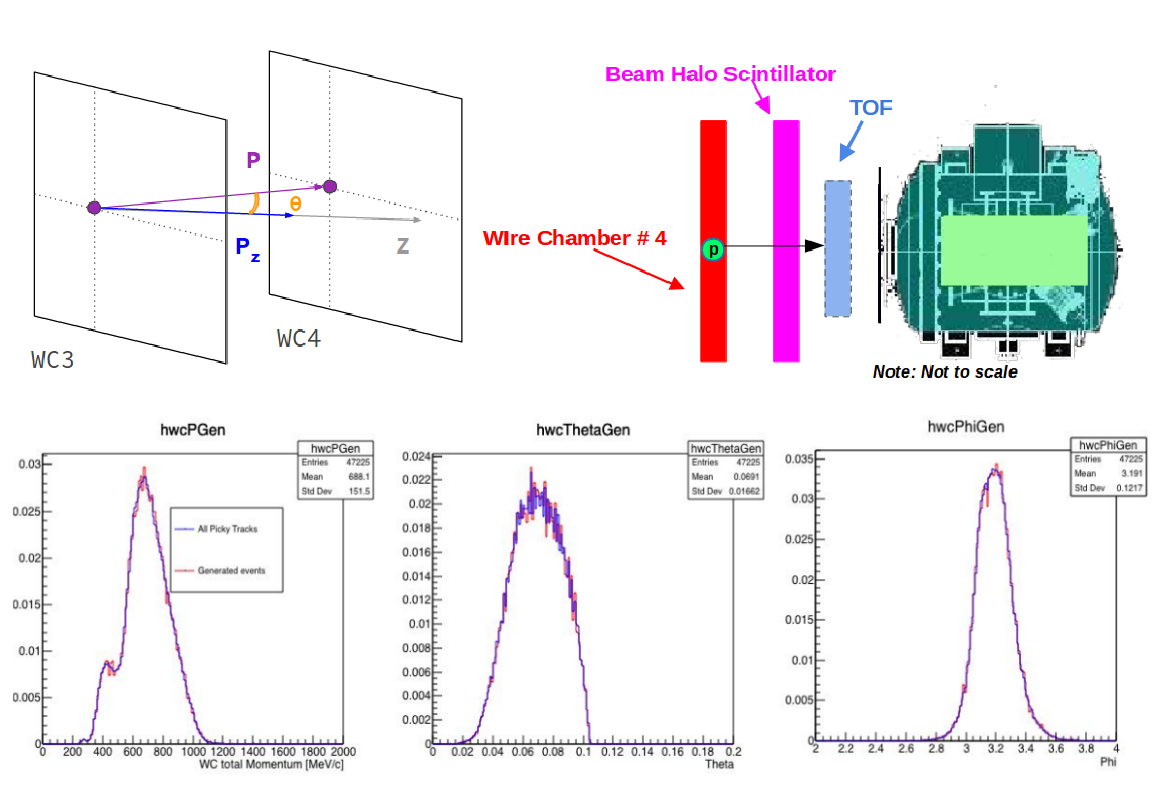
\includegraphics[width=0.70\textwidth]{images/DDMC.png}
\caption{Illustration of the technique where the wire chamber track initial angular and momentum distributions are used to generate the single particle MC.}
\label{fig:DDMC}
\end{figure}

Table \ref{tab:MCSampleGen} lists the various MC samples that were generated for this analysis. 

\begin{table}[htb]
	\begin{center}
	\resizebox{0.95\textwidth}{!}{%
	\begin{tabular}{|c|c|c|}
	\hline
	  \textbf{DDMC Sample} & Original Data Distribution & Number of Events Generated  \\
	  	\hline
	Run-II $\pi^{+}$ & $\pi, \mu, e$ Mass Filter / Picky WC-Track & \\
	Run-II $\mu^{+}$ & $\pi, \mu, e$ Mass Filter / Picky WC-Track &  \\
	Run-II $e^{+}$ & $\pi, \mu, e$ Mass Filter / Picky WC-Track & \\
	Run-II $K^{+}$ & $K^{+}$ Mass Filter / Picky WC-Track & \\
	Run-II $p$ & $p$ Mass Filter / Picky WC-Track & \\
	\hline
	\end{tabular}}
	\caption{Summary of MC generated for the analysis.} \label{tab:MCSampleGen}
	\end{center}
\end{table}

\textcolor{red}{CHECK WITH THE BEAMLINE MC IF WE REALLY NEED THIS}
In addition to this sample of DDMC, a sample of photons is also generated since as is shown in Table \ref{tab:beamcomp1} a small but non-negligible portion of the beam will have photons entering the TPC. This sample is generated with a flat momentum spectrum between 0 MeV and 2000 MeV with a Gaussian angular distribution of $\pm$5 degrees about the beam direction. The photon momentum spectrum is then re-weighted by the momentum spectrum of the corresponding run period it is being simulated for. This approximation allows us to estimate the contamination due to photons from MC with a reasonable assumption of their spectrum.


